\documentclass{article}
\usepackage[utf8]{inputenc}
\usepackage{graphicx}
\usepackage{here}
\usepackage{amsmath}

\title{Notes de cours\\OPT5 : Apprentissage par renforcement}
\author{Adrien Pavao}
\date{Novembre 2017}

\begin{document}

\maketitle

\section{Introduction}

L'apprentissage par renforcement consiste à apprendre à partir d'expériences, plutôt qu'à partir de données pré-établies, de façon à optimiser une récompense quantitative au cours du temps.

Un agent est plongé au sein d'un environnement. Il doit choisir ses actions (prise de décision) en fonction de son état courant. En retour, l'agent reçoit une récompense de l'environnement, qui peut être positive ou négative.

L'agent cherche à améliorer sa politique de décision au fur et à mesure de sorte à maximiser sa récompense.

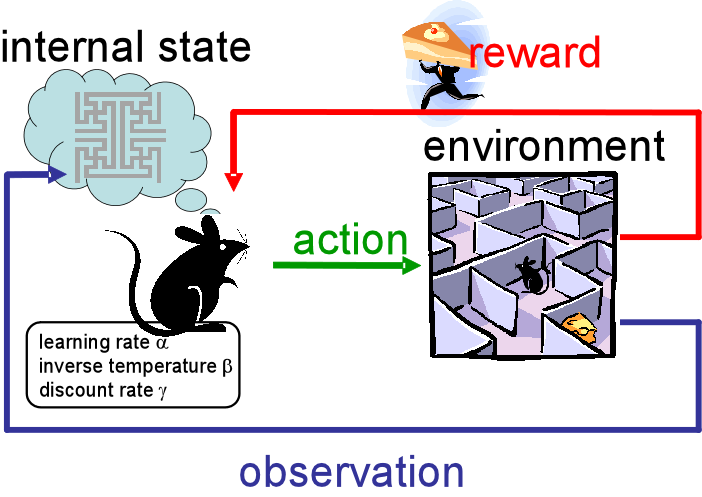
\includegraphics[scale=0.4]{opt5.png}

Dans l'illustration ci-dessus, on voit :
\begin{itemize}
\item \textbf{L'environnement :} Le labyrinthe.
\item \textbf{L'agent :} La souris. C'est l'observation qu'elle fait de l'environnement que l'on nomme son état courant. On nomme tous les états possibles l'\textbf{espace des états}.
\item \textbf{Les actions :} Les actions possibles de la souris en réaction à l'état. Avancer, tourner à gauche, revenir en arrière, etc. Toutes les actions réalisables par l'agent constituent l'\textbf{espace des actions}.
\item \textbf{La récompense :} Le fromage. La souris souhaite tirer profit de sa perception et de sa stratégie de décision afin d'accéder à cette récompense, si possible en un temps minimal.
\end{itemize}

\section{Processus de décision markovien}

Un processus de décision markovien (MDP) est un modèle stochastique où un agent prend des décisions et où les résultats de ses actions sont aléatoires.\footnote{https://fr.wikipedia.org/wiki/Processus\_de\_décision\_markovien}

Formellement, un MDP est un quadruplet ${S, A, T, R}$ :
\begin{itemize}
\item Espace des états S (dénombrable ou continu)
\item Espace des actions A (dénombrable ou continu)
\item Fonction de transition $p(s, a, s') \rightarrow [0, 1]$ (déterministe ou probabiliste)
\item Récompense r(s)
\end{itemize}

On cherche une stratégie $\pi$ qui maximise l'espérance des récompenses cumulées.\\
L'horizon temporelle est notée H et peut être fini (problème épisodique) ou infini (problème coninu).

\section{Equation de Bellman}

\begin{itemize}

\item \textbf{La fonction d'évaluation V} décrit les meilleurs valeurs possibles de l'objectif selon l'état. Le calcul de V nous permet d'avoir également la fonction a(x) decrivant l'action optimale selon l'état : la fonction de politique.

\item \textbf{L'équation de Bellman} est une condition nécessaire d'optimalité. Elle permet de connaitre la fonction d'évaluation V optimale et la politique optimale. 

\end{itemize}
Voici l'équation générale\footnote{https://en.wikipedia.org/wiki/Bellman\_equation} :

% Wiki
%\[ V(s) = max_{a \in \Gamma(x)} (F(x, a) + \Beta V(T(x, a))) \]
\[ V(x) = \max_{a \in \Gamma (x) } \{ F(x,a) + \beta V(T(x,a)) \} \]

Dans le cas des processus de décision de Markov, l'équation de Bellman est une récursion des récompenses attendues :

\[ V(s) = r(s) + \gamma \sum_{s'} p(s, \pi(s), s') V(s') \]

Il s'agit d'une équation fonctionnelle, dont l'inconnue est la fonction V. On voit que cela consiste en la somme de la récompense à l'état s et de $\gamma$ fois la somme des évaluations des états suivants (par la politique $\pi$ et pondéré par les probabilités dans le cas d'un problème non-déterministe). La récursion s'arrête aux états finaux. La \textbf{stratégie optimale} est celle qui maximise V ?

\textbf{Hypothèse.} Dans le cas déterministe : 

\[ V(s) = r(s) + \gamma V(s') \]

\section{Dilemme Exploration Exploitation}

Exemple du bandit manchot. Doit-on exploiter le bras que l'on estime être le meilleur ou bien explorer plus pour peut-être trouver un bras plus rentable ?

\subsection*{Regret}

Dans un problème de bandit manchot, le regret après K essais est défini comme la différence entre la récompense que l'on obtiendrait en utilisant K fois la meilleur machine et l'espérance de la récompense après K essais :

\[ r_K = K\mu^* - \sum_{k=1}^K E(\mu_{I_k}) \]

\subsection*{Inégalité de Hoeffding}

Soit $r_1$, ..., $r_n$ i.i.d. dans [0, 1] ... Voir cours.

\end{document}


